% !TeX TS-program = xelatex

\documentclass[compress, 8pt]{beamer}

\usepackage{presentationtemplate}
\usepackage[askip=3mm, bskip=3mm]{terminal}
\usepackage[linenosfontsize=\tiny, askip=3mm, bskip=3mm]{mylisting}
\usepackage{tikz}
\usetikzlibrary{positioning}
\usepackage{csquotes}

\title{Структуры и классы}

\begin{document}

\frame[plain]{\titlepage}

\begin{frame}[fragile]

    \frametitle{Проблема}

    Некоторые объекты из предметной области программы могут быть представлены
    в ее коде только как набор из двух или более объектов:

    \begin{myinplacelisting}[minted language=cpp]
// комплексное число z = 1 - 2.5i;
double z_real { 1 };
double z_imaginary { -2.5 };

// точка в трехмерном пространстве p (0; 0; -6)
int p_x { 0 };
int p_y { 0 };
int p_z { -6 };
    \end{myinplacelisting}

    Как выразить логическую связь между этими объектами в коде?
    Объединить эти объекты в один можно при помощи пользовательских типов:
    \textbf{структур} и \textbf{классов}\footnotemark{}.

    \footnotetext{\url{https://en.cppreference.com/w/cpp/language/class}}

\end{frame}

\begin{frame}[fragile]

    \frametitle{Объявление и определение структуры}

    Объявление структуры:

    \begin{myinplacelisting}[minted language=cpp]
// объявляем тип для представления комплексного числа
struct ComplexNumber;
    \end{myinplacelisting}

    Объявление структуры с определением:

    \begin{myinplacelisting}[minted language=cpp]
struct ComplexNumber {
    double real;        // действительная часть
    double imaginary;   // мнимая часть
};
    \end{myinplacelisting}

    Создание объекта с типом \verb|ComplexNumber| на стеке:

    \begin{myinplacelisting}[minted language=cpp]
int main() {
    ComplexNumber z;
}
    \end{myinplacelisting}

\end{frame}

\begin{frame}[fragile]

    \frametitle{Поля структуры}

    Перечисленные в определении структуры объекты называются ее
    \textbf{полями}\footnotemark{} (data members).
    Полями структуры могут быть и объекты и других пользовательских типов.

    \footnotetext{\url{https://en.cppreference.com/w/cpp/language/data\_members}}

    \begin{myinplacelisting}[minted language=cpp]
// определяем тип точки на плоскости
struct Point {
    double x;
    double y;
};

// определяем тип отрезка на плоскости
struct Segment {
    Point begin;    // начало отрезка
    Point end;      // конец отрезка
};
    \end{myinplacelisting}

\end{frame}

\begin{frame}[fragile]

    \frametitle{Инициализация}

    Существует большое число способов инициализировать структуру:

    \begin{myinplacelisting}[minted language=cpp]
ComplexNumber z0;   // инициализации нет
                    // поля могут быть заполнены произвольно
ComplexNumber z1 {};
ComplexNumber z2 {0.0, 0.0};
ComplexNumber z3 {.real=0.0, .imaginary=0.0}; // C++20
ComplexNumber z4 = {};
ComplexNumber z5 = {0.0, 0.0};
ComplexNumber z6 = {.real=0.0, .imaginary=0.0}; // C++20
    \end{myinplacelisting}

\end{frame}

\begin{frame}[fragile]

    \frametitle{Обращение к полям структуры}

    \hfill\break
    Обращение на чтение или запись к отдельному полю структуры используется оператор
    \textbf{member of object} (\verb|.|) для объектов и ссылок и оператор
    \textbf{member of pointer} (\verb|->|) для указателей\footnotemark{}.

    \footnotetext{\url{https://en.cppreference.com/w/cpp/language/operator\_member\_access}}

    \myinputlisting[minted language=cpp]
        {Presentations/11-Structs-and-classes/member-data-access/}
        {main.cpp}

\end{frame}

\begin{frame}[fragile]

    \frametitle{Иммутабельность полей}

    \hfill\break
    Если объект объявлен константным, то все его поля защищены от изменений:

    \begin{myinplacelisting}[minted language=cpp]
const ComplexNumber z {};
z.real = -1.0; // ошибка компиляции
    \end{myinplacelisting}

    Можно сделать константным конкретное поле структуры в ее определении:

    \begin{myinplacelisting}[minted language=cpp]
struct S {
    int a;
    const int b;
};

int main() {
    S s; // ошибка компиляции
    S s {0, 1};
    ++s.a;
    ++s.b; // ошибка компиляции
}
    \end{myinplacelisting}

\end{frame}

\begin{frame}[fragile]

    \frametitle{Представление в памяти}

    \begin{columns}[T]

        \begin{column}{0.5\textwidth}

            \myinputlisting[minted language=cpp]
                {Presentations/11-Structs-and-classes/members-order/}
                {main.cpp}

        \end{column}

        \begin{column}{0.5\textwidth}

            \begin{terminalwindow}
!\shellcommand{g++ main.cpp -o main}!
!\shellcommand{./main}!
0x7ffcb6f71a30
24
0x7ffcb6f71a30
0x7ffcb6f71a38
0x7ffcb6f71a40
            \end{terminalwindow}

            Поля структуры расположены в памяти объекта, которому они принадлежат.
            Порядок расположения полей гарантирован и совпадает с порядком их
            объявления в определении структуры.

        \end{column}

    \end{columns}

\end{frame}

\begin{frame}[fragile]

    \frametitle{Выравнивание полей}

    Размер структуры зависит от его суммы размеров её полей, но не обязательно равен ей
    \footnotemark{}.

    \begin{myinplacelisting}[minted language=cpp]
#include <cstdint>

struct Foo {
    std::int32_t a;
    std::int8_t b;
};

int main() {
    // ошибка компиляции
    static_assert(sizeof(Foo) == 5);
    // ок
    static_assert(sizeof(Foo) == 8);
}
    \end{myinplacelisting}

    \footnotetext{Подробнее про \texttt{static\_assert} из кода на листинге см.
        \href{https://en.cppreference.com/w/cpp/language/static\_assert}{тут}.}

\end{frame}

\begin{frame}[fragile]

    \frametitle{Выравнивание полей}

    \break\hfill
    \begin{columns}[T]

        \begin{column}{0.6\textwidth}

            Многие аппаратные платформы накладывают правила на адреса ОЗУ, по которым
            происходит обращение (чтение или запись) к участку памяти определенного
            размера\footnote{Подробнее об особенностях выравнивания полей структур см.
                \href{https://habr.com/ru/articles/142662/}{тут}.}.

            \begin{myinplacelisting}[minted language=cpp]
#include <cstdint>

struct Foo {
    std::uint8_t a;
    std::uint32_t b;
};

int main() {
    Foo f { 0xAA, 0xBBBBBBBB };
}
            \end{myinplacelisting}

        \end{column}

        \begin{column}{0.4\textwidth}

            \hfill\break
            \centering
            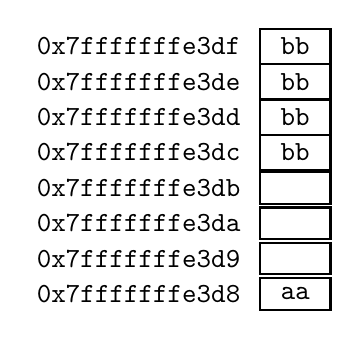
\begin{tikzpicture} [
                bytenode/.style={
                    rectangle,
                    thick,
                    minimum width=9mm,
                    minimum height=4mm
                }
            ]
                \node[bytenode] (addr0)                                 {\verb|0x7fffffffe3d8|};
                \node[bytenode] (addr1) [above=-\pgflinewidth of addr0] {\verb|0x7fffffffe3d9|};
                \node[bytenode] (addr2) [above=-\pgflinewidth of addr1] {\verb|0x7fffffffe3da|};
                \node[bytenode] (addr3) [above=-\pgflinewidth of addr2] {\verb|0x7fffffffe3db|};
                \node[bytenode] (addr4) [above=-\pgflinewidth of addr3] {\verb|0x7fffffffe3dc|};
                \node[bytenode] (addr5) [above=-\pgflinewidth of addr4] {\verb|0x7fffffffe3dd|};
                \node[bytenode] (addr6) [above=-\pgflinewidth of addr5] {\verb|0x7fffffffe3de|};
                \node[bytenode] (addr7) [above=-\pgflinewidth of addr6] {\verb|0x7fffffffe3df|};
                \node[bytenode, draw] (b0) [right=1mm of addr0] {\verb|aa|};
                \node[bytenode, draw] (b1) [right=1mm of addr1] {};
                \node[bytenode, draw] (b2) [right=1mm of addr2] {};
                \node[bytenode, draw] (b3) [right=1mm of addr3] {};
                \node[bytenode, draw] (b4) [right=1mm of addr4] {\verb|bb|};
                \node[bytenode, draw] (b5) [right=1mm of addr5] {\verb|bb|};
                \node[bytenode, draw] (b6) [right=1mm of addr6] {\verb|bb|};
                \node[bytenode, draw] (b7) [right=1mm of addr7] {\verb|bb|};
            \end{tikzpicture}

        \end{column}

    \end{columns}

\end{frame}

\begin{frame}[fragile]

    \frametitle{Статические поля}

    Поле структуры может иметь статическое время хранения.

    \begin{myinplacelisting}[minted language=cpp]
#include <iostream>

struct Foo {
    static unsigned a;
};

unsigned Foo::a = 0;

int main() {
    Foo foo1 {};
    foo1.a = 1;

    Foo foo2 {};
    // выведет 1
    std::cout << foo2.a << std::endl;
}
    \end{myinplacelisting}

\end{frame}

\begin{frame}[fragile]

    \frametitle{Методы}

    \hfill\break
    Определение структуры может содержать функции, называемые
    \textbf{методами}\footnotemark{} (member functions).
    Область видимости определений методов включает все поля структуры.

    \footnotetext{\url{https://en.cppreference.com/w/cpp/language/member\_functions}}

    \begin{myinplacelisting}[minted language=cpp]
#include <cmath>

struct ComplexNumber {
    double real;
    double imaginary;
    double Modulus() {
        const double squares_sum =
            std::pow(real, 2) +
            std::pow(imaginary, 2);
        return std::sqrt(squares_sum);
    }
    void Multiply(const double number) {
        real *= number;
        imaginary *= number;
    }
};
    \end{myinplacelisting}

\end{frame}

\begin{frame}[fragile]

    \frametitle{Определения методов}

    Методы, определенные внутри класса, являются встраиваемыми.
    Чаще всего нужно определять методы вне класса, чтобы потенциально
    уменьшить размер бинарного файла.

    \begin{columns}[T]

        \begin{column}{0.4\textwidth}

            \myinputlisting[minted language=cpp]
                {Presentations/11-Structs-and-classes/method-definition/}
                {complex-number.hpp}

        \end{column}

        \begin{column}{0.6\textwidth}

            \myinputlisting[minted language=cpp]
                {Presentations/11-Structs-and-classes/method-definition/}
                {complex-number.cpp}

        \end{column}

    \end{columns}

\end{frame}

\begin{frame}[fragile]

    \frametitle{Константные методы}

    \hfill\break
    Метод может быть объявлен с квалификатором \verb|const|.
    В теле такого метода не может быть изменения полей структуры.
    Методы без \verb|const| не могут быть вызваны у неконстантных объектов.

    \begin{myinplacelisting}[minted language=cpp]
#include <cmath>

struct ComplexNumber {
    // поля структуры...
    double Modulus() const;
    void Multiply(const double number);
};

double ComplexNumber::Modulus() const {/*...*/}
void ComplexNumber::Multiply(const double number)
{/*...*/}

int main() {
    const ComplexNumber number {};
    number.Multiply(2.0); // ошибка компиляции
    const double mod = number.Modulus();
}
    \end{myinplacelisting}

\end{frame}

\begin{frame}[fragile]

    \frametitle{Указатель \texttt{this}}

    \hfill\break
    Внутри определений методов можно пользоваться ключевым словом
    \verb|this|\footnotemark{},
    которое \enquote{раскроется} в указатель на текущий объект.

    \footnotetext{\url{https://en.cppreference.com/w/cpp/language/this}}

    \begin{myinplacelisting}[minted language=cpp]
struct ComplexNumber {
    double real;
    double imaginary;
    ComplexNumber& Add(const ComplexNumber& o) {
        this->real += o.real;
        this->imaginary += o.real;
        return *this;
    }
};

int main() {
    ComplexNumber z0 {1.0, -1.0};
    ComplexNumber z1 {-2.0, 2.0};
    ComplexNumber z2 {0.0, -3.0};
    ComplexNumber z3 {};
    z3.Add(z0).Add(z1).Add(z2);
}
    \end{myinplacelisting}

\end{frame}

\begin{frame}[fragile]

    \frametitle{Операторы}

    Методом структуры может являться оператор.

    \begin{myinplacelisting}[minted language=cpp]
struct ComplexNumber {
    double real;
    double imaginary;
    ComplexNumber& operator*=(const double number) {
        real *= number;
        imaginary *= number;
        return *this;
    }
};

int main() {
    ComplexNumber z {1.0, -1.0};
    z *= 2.0;
}
    \end{myinplacelisting}

\end{frame}

\begin{frame}[fragile]

    \frametitle{Операторы}

    Пример оператора сложения для \verb|ComplexNumber|.

    \begin{myinplacelisting}[minted language=cpp]
struct ComplexNumber {
    double real;
    double imaginary;
    ComplexNumber operator+(const ComplexNumber& o) {
        ComplexNumber result {
            real + o.real,
            imaginary + o.imaginary
        };
        return result;
    }
};

int main() {
    ComplexNumber z0 {1.0, -1.0};
    ComplexNumber z1 {-2.0, 2.0};
    ComplexNumber z2 {0.0, -3.0};
    ComplexNumber z3 { z0 + z1 + z2 };
}
    \end{myinplacelisting}

\end{frame}

\begin{frame}[fragile]

    \frametitle{Спецификаторы доступа}

    \hfill\break
    Внутри определения класса могут находиться спецификаторы
    доступа\footnote{\url{https://en.cppreference.com/w/cpp/language/access}}
    \verb|public|, \verb|private| и \verb|protected|\footnotemark{}.

    \footnotetext{Спецификатор \texttt{protected} будет рассмотрен позднее при изучении
        наследования структур и классов.}

    \begin{itemize}
        \item Доступ к полям и методам под спецификатором \verb|public| не
            ограничивается.
        \item Доступ к полям и методам под спецификатором \verb|private|
            ограничен определениями методов.
    \end{itemize}

    \begin{myinplacelisting}[minted language=cpp]
struct ComplexNumber {
private:
    double real, imaginary;
public:
    ComplexNumber& operator*=(const double number);
};

int main() {
    ComplexNumber z {};
    z *= 2.0; // ок
    const double r = z.real; // ошибка компиляции
}
    \end{myinplacelisting}

\end{frame}

\begin{frame}[fragile]

    \frametitle{Классы и структуры}

    В классе все поля и методы по-умолчанию \verb|private|, а в структуре
    --- \verb|public|.

    \begin{columns}[T]

        \begin{column}{0.5\textwidth}

            \begin{myinplacelisting}[minted language=cpp]
struct Date {
    // неявно public
    bool SetDay(unsigned);
    bool SetMonth(unsigned);
    bool SetYear(unsigned);
private:
    unsigned day_;
    unsigned month_;
    unsigned year_;
};
            \end{myinplacelisting}

        \end{column}

        \begin{column}{0.5\textwidth}

            \begin{myinplacelisting}[minted language=cpp]
class Date {
    // неявно private
    unsigned day_;
    unsigned month_;
    unsigned year_;
public:
    bool SetDay(unsigned);
    bool SetMonth(unsigned);
    bool SetYear(unsigned);
};
            \end{myinplacelisting}

        \end{column}

    \end{columns}

\end{frame}

\begin{frame}[fragile]

    \frametitle{Конструктор и деструктор}

    Специальные методы, отвечающие за создание и уничтожение объектов, называются
    \textbf{конструктор} (конструктор)\footnote{\url{https://en.cppreference.com/w/cpp/language/constructor}}
    и \textbf{деструктор} (деструктор)\footnote{\url{https://en.cppreference.com/w/cpp/language/destructor}}.

    Эти методы вызываются автоматически в моменты начала и конца времени жизни объекта.

    \begin{myinplacelisting}[minted language=cpp]
struct Foo {
    Foo() {} // конструктор
    ~Foo() {} // деструктор
};

void bar(const bool condition) {
    Foo foo {}; // вызывается конструктор
    if (condition) {
        return; // вызывается деструктор
    }
} // вызывается деструктор
    \end{myinplacelisting}

\end{frame}

\begin{frame}[fragile]

    \frametitle{Параметры конструктора}

    \hfill\break
    Как и любая функция, конструктор может иметь параметры и принимать
    аргументы.
    Чаще всего параметры конструктора нужны для инициализации полей класса.

    \begin{myinplacelisting}[minted language=cpp]
class ComplexNumber {
public:
    ComplexNumber(const double real, const double imaginary):
        real_(real), imaginary_(imaginary)
    {}
private:
    const double real_, imaginary_;
};

int main() {
    ComplexNumber z0(1.0, 2.0); // старый (C++98) вариант
                                // инициализации с
                                // конструктором
    ComplexNumber z1 {1.0, 2.0};
    ComplexNumber z2 {}; // ошибка компиляции
}
    \end{myinplacelisting}

\end{frame}

\begin{frame}[fragile]

    \frametitle{Несколько конструкторов}

    \hfill\break
    Конструкторов класса может быть несколько.

    \begin{myinplacelisting}[minted language=cpp]
class ComplexNumber {
public:
    ComplexNumber();
    ComplexNumber(const double real, const double imaginary);
private:
    const double real_, imaginary_;
};

ComplexNumber::ComplexNumber(
    const double real, const double imaginary) :
    real_(real), imaginary_(imaginary)
{}

ComplexNumber::ComplexNumber() :
    real_(0.0), imaginary_(0.0) {}

int main() {
    ComplexNumber z0 {1.0, 2.0};
    ComplexNumber z1 {};
}
    \end{myinplacelisting}

\end{frame}

\begin{frame}[fragile]

    \frametitle{Деструктор}

    Конструктор и деструктор работают в паре для аллокации и деаллокации
    каких-либо ресурсов (память в куче, открытие/закрытие файлов и т.д.).
    Такая привязка ресурса к времени жизни объекта называется \textbf{RAII}\footnotemark{}
    (Resource Acquisition Is Initialization).

    \footnotetext{\url{https://en.cppreference.com/w/cpp/language/raii},
        \url{https://en.wikipedia.org/wiki/Resource\_acquisition\_is\_initialization}}

    \begin{myinplacelisting}[minted language=cpp]
#include <cstddef>

class DynamicArray {
public:
    DynamicArray(const std::size_t size) :
        size_(size), ptr_(new int[size]) {}
    ~DynamicArray() {
        delete [] ptr_;
    }
private:
    std::size_t size_;
    int* ptr_;
};
    \end{myinplacelisting}

\end{frame}

\end{document}
